\documentclass[11pt]{article}
\usepackage[final]{acl}
\usepackage{times}
\usepackage{latexsym}
\usepackage[T1]{fontenc}
\usepackage[utf8]{inputenc}
\usepackage{microtype}
\usepackage{inconsolata}
\usepackage{graphicx}
\usepackage{booktabs}
\usepackage{amsmath}
\usepackage{multirow}

\title{Multi-Signal Interpretability Identifies Task-Critical Circuits\\for Efficient Model Compression}

  \author{Srikar Vardhan Mangadoddi \\
    National Institute of Technology Silchar \\
    Petavue \\
    \texttt{srikar@petavue.com}}

\begin{document}
\maketitle

\begin{abstract}
Post-training quantization methods such as GPTQ and AWQ minimize 
reconstruction error without asking which weights matter for the 
task. We combine six interpretability signals to select a sparse 
skeleton of task-critical MLP neurons that is kept at 16-bit while 
the rest of the model is quantized. On Gemma-2-2B fine-tuned for 
SQL generation, the 0.54\% skeleton with 3-bit MLPs and 8-bit 
attention retains \textbf{100\% of baseline-correct outputs at 
4.03$\times$ compression}, versus 75.2\% for uniform 4-bit. On 
Llama-3-8B fine-tuned for Cypher generation, where uniform 4-bit 
loses 23 points, the 0.46\% skeleton recovers 14.4 of them and a 
random skeleton of equal size recovers none. Three signals are 
individually effective and three are not, and the effective set 
differs between models, so the consensus rule provides robustness 
no single signal does. Selection matters where uniform 
quantization leaves headroom, which suggests measuring headroom, 
selecting by consensus, and protecting as a recipe for larger 
models. GPTQ error compensation degrades 3-bit layouts by 16 to 
18 points regardless of protection.
\end{abstract}

\section{Introduction}
Fine-tuned language models are now the standard deployment 
unit: practitioners routinely adapt base models to tasks such as 
code generation, summarization, or SQL synthesis, and deploying 
them in resource-constrained settings requires compression. 
Post-training quantization methods such as GPTQ 
\cite{frantar2023gptqaccurateposttrainingquantization} and AWQ 
\cite{lin2024awqactivationawareweightquantization} lower weight 
precision effectively, but they minimize reconstruction error 
without asking \emph{which neurons matter for the task}.

Fine-tuning creates task-specific computational pathways, 
circuits in the loose sense of neuron subsets critical for a 
learned capability \cite{olah2020zoom,elhage2021mathematical}, 
and these changes are sparse and localized 
\cite{panigrahi2023taskspecificskilllocalizationfinetuned,
prakash2024finetuningenhancesexistingmechanisms}. If we can 
identify this circuit, we can protect it at full precision and 
compress everything else. TaCQ 
\cite{xiao2025taskcircuitquantizationleveragingknowledge} takes 
a step in this direction with weight-perturbation and gradient 
signals at weight granularity. We ask a simpler question first: 
does the choice of protected neurons matter at all, and if so, 
which signals identify them?

We propose \textbf{CircuitTier}, which combines six 
interpretability signals (Figure~\ref{fig:pipeline}) to select 
a sparse skeleton of task-critical MLP neurons that is kept at 
16-bit while the remaining weights are quantized. The signals 
have low top-$k$ overlap (mean Jaccard of top-1,295 neurons: 
0.012), so each identifies neurons the others rank as 
unimportant.\footnote{Code, results, and an interactive 3D 
circuit explorer are available at \url{https://github.com/M-SRIKAR-VARDHAN/circuittier}.} On 
Gemma-2-2B \cite{gemmateam2024gemma2improvingopen} fine-tuned on 
TinySQL \cite{harrasse2025tinysqlprogressivetexttosqldataset}, 
the 0.54\% skeleton at 16-bit with 3-bit MLPs and 8-bit 
attention retains 100\% of baseline-correct outputs at 
4.03$\times$ compression, versus 75.2\% for uniform 4-bit. On 
this model the precision layout does the work: the same 
retention is reached with no skeleton, because low-bit MLPs 
with 8-bit attention leave nothing to recover. On Llama-3-8B 
\cite{grattafiori2024llama3herdmodels} fine-tuned for Cypher 
generation \cite{ozsoy2024text2cypherbridgingnaturallanguage}, 
uniform 4-bit loses 23 points and the skeleton matters: 
protecting the 0.46\% our signals select recovers 14.4 points, 
while a random skeleton of the same size recovers none. 
Selection matters where uniform quantization leaves headroom, 
which suggests measuring headroom, selecting by consensus, and 
protecting as a recipe for larger and harder-to-quantize models.

Our contributions are:
\begin{enumerate}
\itemsep0em
\item A framework that selects a sparse skeleton from six 
interpretability signals at neuron granularity, reaching 100\% 
task retention at 4.03$\times$ on Gemma-2-2B.
\item Evidence that the identity of protected neurons matters 
when the compressed model has something to lose: on Llama-3-8B 
the multi-signal skeleton recovers 14.4 points over uniform 
4-bit while random protection recovers 0.0 ($n{=}894$). Three 
signals are individually effective and three are not, the 
effective set differs between models, and the consensus rule 
matches the best single signal on both without knowing which it 
is.
\item Two negative results: GPTQ error compensation degrades 
3-bit layouts by 16 to 18 points regardless of protection while 
helping at 4-bit, and zeroing the neurons all six signals rank 
lowest costs 8 points.
\end{enumerate}


\section{Related Work}
Post-training quantization methods reduce weight precision 
without retraining: GPTQ 
\cite{frantar2023gptqaccurateposttrainingquantization} uses 
second-order information, AWQ 
\cite{lin2024awqactivationawareweightquantization} protects 
salient weights via activation magnitudes, and SpQR 
\cite{dettmers2023spqrsparsequantizedrepresentationnearlossless} 
isolates outlier weights. Mixed-precision methods such as HAWQ 
\cite{dong2019hawqhessianawarequantization} assign bit-widths 
per layer via Hessian sensitivity, while OWQ 
\cite{lee2024owqoutlierawareweightquantization} and SqueezeLLM 
\cite{kim2024squeezellmdenseandsparsequantization} operate per 
weight group. These methods use one or two mathematical criteria 
at weight or layer granularity and are task-agnostic by design.

On the interpretability side, LLM-Pruner 
\cite{ma2023llmprunerstructuralpruninglarge} uses gradients to 
identify removable structures and ShortGPT 
\cite{men2024shortgptlayerslargelanguage} removes layers by 
importance. Pruning-at-initialization methods such as SNIP 
\cite{lee2019snipsingleshotnetworkpruning}, GraSP 
\cite{wang2020pickingwinningticketstraining}, and SynFlow 
\cite{tanaka2020pruningneuralnetworksdata} score parameters of 
an untrained network to select a trainable subnetwork; we 
instead operate on an already fine-tuned model and target the 
circuit introduced by fine-tuning, using signals that presuppose 
a base checkpoint. Circuit discovery methods 
\cite{conmy2023automatedcircuitdiscoverymechanistic,
syed2023attributionpatchingoutperformsautomated} locate the 
components responsible for a behavior; we use one of them, 
attribution patching, as a signal.Analyses of what fine-tuning changes report that it strengthens existing mechanisms rather than building new ones \cite{prakash2024finetuningenhancesexistingmechanisms}, that 
its effect is localized to a small fraction of parameters 
\cite{panigrahi2023taskspecificskilllocalizationfinetuned}, 
and that it can be reverted by editing a sparse set of 
components \cite{jain2024mechanisticallyanalyzingeffectsfinetuning}; 
these motivate looking for a sparse protected set at all. Most closely related, TaCQ \cite{xiao2025taskcircuitquantizationleveragingknowledge} 
combines weight magnitude, gradient, and quantization-effect 
terms into a single per-weight saliency score. Its components 
derive from the same backward pass and are correlated by 
construction, with binary protection at weight granularity. We 
use six independently computed signals at neuron granularity, 
compare fine-tuned and base model weights and activations to 
isolate task-specific circuits, and, unlike prior work, test 
whether the selected neurons matter against random selection of 
equal size.


\begin{figure*}[t]
\centering
\includegraphics[width=\textwidth, trim=40 20 40 20, clip]{figures/fig1_pipeline.jpg}
\caption{We analyze the fine-tuned and base models using six 
interpretability signals, each revealing a different aspect of 
neuron importance. Signals are combined via consensus rules to 
classify the 239,616 MLP neurons of Gemma-2-2B into precision 
tiers; the main configuration keeps the skeleton tier at 16-bit 
and quantizes all remaining MLP weights to 3-bit and attention 
to 8-bit.}
\label{fig:pipeline}
\end{figure*}

\section{Method}
Our approach rests on a simple premise: fine-tuning creates 
task-specific circuits. By comparing the fine-tuned model 
against its base checkpoint, we identify which neurons the 
model relies on for the target task and protect them during 
compression, in three stages (Figure~\ref{fig:pipeline}): signal 
extraction, tier classification, and mixed-precision 
quantization. Throughout, a \emph{neuron} is a single MLP 
intermediate dimension: one row of the gate and up projections 
and the corresponding column of the down projection, the atomic 
unit at which we assign precision.

\subsection{Signal Extraction}

We compute six interpretability signals for all 239,616 MLP 
neurons and 208 attention heads (Table~\ref{tab:signals}). 
\emph{EAP} zero-ablates each neuron and records the change in 
the target-token logit, on 50 analysis samples. \emph{Gradient 
saliency} accumulates the absolute loss gradient over each 
neuron's weights on 20 samples. \emph{Weight magnitude} is the 
mean absolute value of the neuron's weights and needs no data. 
\emph{Weight delta} is the mean absolute change in those 
weights between the base and fine-tuned checkpoints. 
\emph{Activation delta} is the change in the neuron's maximum 
activation between the two models over 500 samples. \emph{Edge 
importance} sums the patching scores of all attention-head 
edges into the neuron, capturing connectivity the other five 
per-neuron signals miss. Signals (4) and (5) require both 
checkpoints, isolating task-specific computation from 
general-purpose behavior; the method therefore assumes access 
to the pre-fine-tuning weights. Full definitions are in 
Appendix~\ref{app:signals}.

\begin{table}[t]
\centering
\small
\begin{tabular}{lll}
\toprule
\textbf{\#} & \textbf{Signal} & \textbf{Measures} \\
\midrule
1 & EAP \cite{syed2023attributionpatchingoutperformsautomated} & Causal importance \\
2 & Gradient Saliency & Loss sensitivity \\
3 & Weight Magnitude & Parameter scale \\
4 & Weight Delta$^\dagger$ & Fine-tuning change \\
5 & Activation Delta$^\dagger$ & Behavioral shift \\
6 & Edge Importance & Circuit connectivity \\
\bottomrule
\end{tabular}
\caption{Six interpretability signals, each min-max normalized 
to $[0,1]$. $^\dagger$Requires the base checkpoint. Mean 
pairwise Pearson $|r|{=}0.098$ (Magnitude and Weight~$\Delta$: 
$r{=}0.85$); mean Jaccard overlap of top-1,295 neurons 0.012. 
Definitions in Appendix~\ref{app:signals}.}
\label{tab:signals}
\end{table}

\subsection{Tier Classification}
\label{sec:tiers}

For each neuron's normalized profile $\{s_1, \ldots, s_6\}$: 
\textbf{Skeleton (16-bit):} $\geq$3 signals exceed 
$\tau{=}0.3$, or EAP $\geq \tau$ with Gradient or 
Activation~$\Delta \geq \tau$ (1,295 neurons, 0.54\%). 
\textbf{Supporting (8-bit):} $\geq$1 signal exceeds $\tau$ with 
a causal signal $\geq 0.2$ (23 neurons). 
\textbf{Prunable (0-bit):} all signals below $\tau'{=}0.1$ 
(48 neurons). \textbf{Compressible:} the remaining 238,250 
(99.4\%). Our main configuration uses only the skeleton tier; 
Section~\ref{sec:findings} shows the supporting tier adds 
nothing and zeroing the prunable tier is harmful.

Because raw signal magnitudes differ across model families, we 
also use a percentile rule: each signal is thresholded at its 
$P$-th percentile and the same consensus applied. On 
Gemma-2-2B, $P{=}99$ and $P{=}99.5$ select 137 and 51 neurons 
and both retain 99.0\% (Section~\ref{sec:selection}); on 
Llama-3-8B, $P{=}99$ selects 2,133 (0.46\%), the skeleton used 
in Section~\ref{sec:llama}.
\subsection{Mixed-Precision Quantization}
\label{sec:quant}
We use per-group round-to-nearest (RTN) quantization with group 
size 128 over each full weight matrix, then restore protected 
neurons from the original weights, so the grouping is identical 
regardless of which neurons are protected. Attention is 
quantized uniformly at 8-bit in the main configuration, since 
attention precision is the dominant factor on Gemma-2-2B 
(Section~\ref{sec:findings}) and 208 heads are too few to tier. 
We write c3+a8 for skeleton at 16-bit, all other MLP weights at 
3-bit, and attention at 8-bit.

\section{Experiments}
\subsection{Setup}

\label{sec:setup}
We fine-tune Gemma-2-2B \cite{gemmateam2024gemma2improvingopen} 
on TinySQL \cite{harrasse2025tinysqlprogressivetexttosqldataset} 
(Appendix~\ref{app:details}) and use the 105 evaluation samples 
it answers correctly, spanning five complexity levels, as the 
retention test set; signals are computed on a disjoint 500-sample 
analysis split. \emph{Retention} is the percentage of these 105 
preserved after compression, by exact match of the first 
generated line under greedy decoding (95\% intervals in 
Appendix~\ref{app:ci}). Compression ratio is $16/\bar{b}$ over 
linear weights, excluding embeddings and norms.

All Gemma and Llama results in this paper use the same 
quantizer and evaluation; the sole exception is the earlier 
protocol of Appendices~\ref{app:ablation} 
and~\ref{app:wall}, which is marked wherever it appears.

\subsection{Main Results}
\label{sec:main}


\begin{table}[t]
\centering
\small
\setlength{\tabcolsep}{4pt}
\resizebox{\columnwidth}{!}{%
\begin{tabular}{lccr}
\toprule
\textbf{Method} & \textbf{Bits} & \textbf{Ratio} & \textbf{Ret.\%} \\
\midrule
Baseline 16-bit & 16.00 & 1.00$\times$ & 100.0 \\
Uniform 4-bit & 4.00 & 4.00$\times$ & 75.2 \\
Uniform 3-bit & 3.00 & 5.33$\times$ & 87.6 \\
GPTQ uniform 4-bit & 4.00 & 4.00$\times$ & 96.2 \\
GPTQ uniform 3-bit & 3.00 & 5.33$\times$ & 77.1 \\
\midrule
MLP@4 + attn@8, no skeleton & 4.73 & 3.38$\times$ & 100.0 \\
CircuitTier c4+a8 & 4.78 & 3.35$\times$ & 99.0 \\
MLP@3 + attn@8, no skeleton & 3.91 & 4.09$\times$ & 98.1 \\
\textbf{CircuitTier c3+a8} & \textbf{3.97} & \textbf{4.03$\times$} & \textbf{100.0} \\
GPTQ MLP@3 + attn@8 ($\pm$ skel.) & 3.97 & 4.03$\times$ & 81.9 \\
\midrule
\multicolumn{4}{l}{\textit{(b) Skeleton selection at c3+a8 (1,295 neurons @16)}} \\
None & & & 98.1 \\
Random (5 seeds) & & & 98.7$\pm$0.5 \\
TaCQ vulnerability top-1,295 & & & 98.1 \\
Percentile $P{=}99$ (137 neurons) & & & 99.0 \\
Six-signal tier rule & & & 100.0 \\
\bottomrule
\end{tabular}}
\caption{(a) Compression and (b) skeleton selection on 
Gemma-2-2B ($n{=}105$). c$b$+a$b'$: skeleton at 16-bit, other 
MLP weights at $b$-bit, attention at $b'$-bit. GPTQ uses damping 
0.01. Rows of (b) differ only in which neurons are restored.}
\label{tab:main}
\end{table}

\begin{figure}[t]
\centering
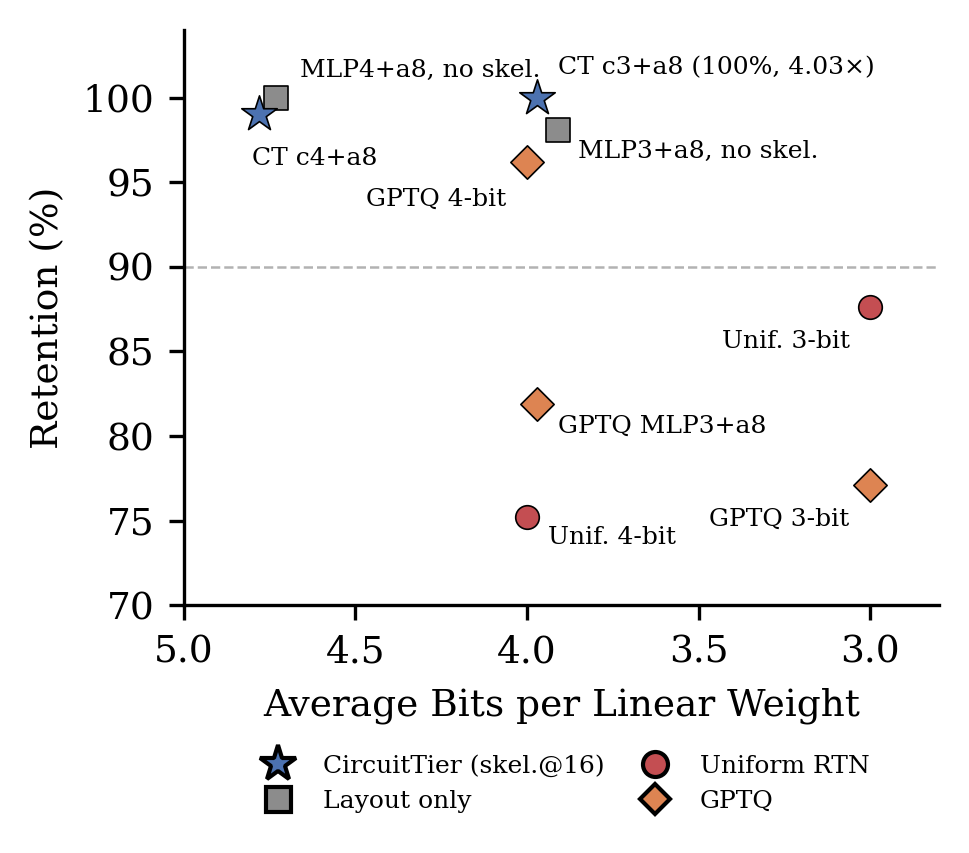
\includegraphics[width=\columnwidth]{figures/fig2_pareto_curve.png}
\caption{Compression and retention on Gemma-2-2B. Squares: no 
neuron protection; stars: with the 0.54\% skeleton. Points 
correspond to rows of Table~\ref{tab:main}(a).}
\label{fig:pareto}
\end{figure}

Uniform 4-bit loses a quarter of correct outputs 
(Table~\ref{tab:main}a). Moving attention to 8-bit and MLPs to 
4-bit recovers all of them at 4.73 bits without protecting any 
neuron. At 3-bit MLPs with 8-bit attention, retention is 98.1\% 
with no skeleton and 100\% with the 0.54\% skeleton at 3.97 
bits (4.03$\times$), against 75.2\% for uniform 4-bit at 4.00 
bits. GPTQ helps uniform 4-bit (96.2\%) but reverses at 3-bit: 
77.1\% uniform and 81.9\% at c3+a8, with or without the 
skeleton.

\subsection{Skeleton Selection}
\label{sec:selection}
Table~\ref{tab:main}(b) fixes the layout at c3+a8 and varies 
only which 1,295 neurons are restored. Every choice, including 
none, lands within two samples of the six-signal rule, which is 
noise at $n{=}105$. The tier-rule skeleton is never worse and 
costs 0.06 bits per weight, so we keep it as a safeguard, but 
on this model selection cannot drive retention: unprotected 
3-bit MLPs already retain 98.1\%, leaving nothing to recover. 
Section~\ref{sec:llama} asks the same question where uniform 
quantization does leave headroom.

\subsection{Key Findings}
\label{sec:findings}

\paragraph{Layout dominates.}
With 4-bit attention, retention is 75.2\% (uniform) and 77.1\% 
(with skeleton); with 8-bit attention, every MLP bit-width from 
3 to 4 retains 98 to 100\%. WikiText-2 perplexity follows suit 
(Appendix~\ref{app:ppl}): MLP@4 with 8-bit attention degrades 
it by 1.05$\times$ against 1.13$\times$ for uniform 4-bit, and 
c3+a8 by 1.47$\times$. The interaction is not monotone in 
bit-width: with 4-bit attention, MLPs at 3-bit retain 95.2\% 
while MLPs at 4-bit retain 75.2\% (uniform 4-bit), and uniform 
3-bit (87.6\%) likewise exceeds uniform 4-bit. We do not have 
an explanation; the practical consequence is that uniform 
4-bit is a weak baseline on this model, and layouts should 
also be compared against uniform 3-bit.

\paragraph{The prunable tier is harmful.}
Zeroing the 48 neurons all six signals rank lowest drops c4+a8 
from 99.0\% to 91.4\%, six of the nine losses in the simplest 
level. Neurons every signal calls unimportant are not safely 
removable.

\paragraph{GPTQ at 3-bit.}
GPTQ improves uniform 4-bit from 75.2\% to 96.2\% but degrades 
every 3-bit layout: uniform 3-bit from 87.6\% to 77.1\%, c3+a8 
from 100\% to 81.9\% with and without the skeleton. Restored 
skeleton columns receive a mean $|\Delta w|$ of 0.00029 from 
error redistribution against 0.00074 for quantized columns, so 
the cause is not contamination of protected weights. GPTQ is 
also sensitive to Hessian conditioning: uniform 4-bit gives 
96.2\% at damping 0.01, 88.6\% at 0.1, and 79.0\% with the same 
code on a different GPU (Appendix~\ref{app:gptq}). We treat the 
3-bit degradation as robust and the 4-bit numbers as indicative.
\section{Does Selection Matter? Llama-3-8B on Cypher}
\label{sec:llama}

Because unprotected low-bit MLPs on Gemma-2-2B retain nearly 
everything, no skeleton can show an effect there. We repeat the 
selection experiment on a model where uniform quantization 
leaves headroom.

\paragraph{Setup.}
We fine-tune Meta-Llama-3-8B 
\cite{grattafiori2024llama3herdmodels} on Cypher generation 
with the Neo4j Text2Cypher 2024 dataset 
\cite{ozsoy2024text2cypherbridgingnaturallanguage} (39,554 
train, 4,833 test; Appendix~\ref{app:details}), reaching 
42.27\% exact match and 2,043 baseline-correct samples. We 
evaluate 1,000 of these by index; batched decoding reproduces 
894 at 16-bit, and retention is relative to those 894. The 
skeleton is the 99th-percentile consensus of 
Section~\ref{sec:tiers}: 2,133 neurons (0.46\%). The layout is 
uniform 4-bit on all projections with only the skeleton 
restored (4.05 bits, 3.96$\times$), so rows differ only in 
which neurons are restored.

\begin{table}[t]
\centering
\small
\begin{tabular}{lr}
\toprule
\textbf{Restored to 16-bit (2,133 neurons)} & \textbf{Ret.\%} \\
\midrule
None (uniform 4-bit) & 77.1 \\
Random, 3 seeds & 77.0$\pm$0.1 \\
\midrule
Weight $\Delta$ & 77.1 \\
Activation $\Delta$ & 77.5 \\
Edge & 76.8 \\
EAP & 90.6 \\
Magnitude & 91.4 \\
Gradient & 91.9 \\
\midrule
\textbf{Six-signal consensus} & \textbf{91.5} \\
\bottomrule
\end{tabular}
\caption{Llama-3-8B, $n{=}894$. Every row is uniform 4-bit 
per-group RTN with 2,133 MLP neurons restored to 16-bit; single 
signals restore their top-2,133. Intervals are no wider than 
3 points (Appendix~\ref{app:ci}).}
\label{tab:llama}
\end{table}

\paragraph{Results.}
Here the identity of the protected neurons matters 
(Table~\ref{tab:llama}). Uniform 4-bit retains 77.1\%; a random 
0.46\% changes nothing (77.0$\pm$0.1); the six-signal skeleton 
recovers 14.4 points to 91.5\%.The 95\% intervals do not overlap: 74.2 to 79.7 for no skeleton against 89.5 to 93.2 for the consensus skeleton 
(Appendix~\ref{app:ci}). The gain falls on the harder 
classes: retained counts rise from 124 to 165 of 177 on CY3, 66 
to 93 of 113 on CY4, and 142 to 183 of 211 on CY5, while CY1 
and CY2 are near ceiling throughout. The single signals split 
cleanly: EAP, magnitude, and gradient each select an effective 
skeleton (90.6 to 91.9\%); weight delta, activation delta, and 
edge are indistinguishable from random. The consensus matches 
the best single signal without exceeding it. Its value is 
robustness: on Gemma-2-2B weight delta was among the strongest 
signals and magnitude among the weakest 
(Appendix~\ref{app:ablation}), so which signals work is not 
predictable, and consensus lands at the effective level on both 
models. Effective skeletons are also not unique: the gradient 
skeleton shares only 623 of 2,133 neurons with the consensus 
yet performs the same. Beyond this layout, no configuration 
between 4.6$\times$ and 9.3$\times$ retains more than 73\% 
(Appendix~\ref{app:wall}).

\paragraph{Recipe.}
The two models together suggest a procedure. First, quantize 
uniformly at the target bit-width and measure retention; this 
is one evaluation and tells you the headroom. If retention is 
already near the 16-bit baseline, as on Gemma-2-2B, spend the 
remaining budget on attention precision and stop. If it is 
not, as on Llama-3-8B, extract the six signals, select the 
skeleton by percentile consensus, restore it to 16-bit, and 
re-evaluate. On Llama-3-8B the second step costs 0.05 bits per 
weight and recovers 14.4 of the 23 points lost. Nothing in the 
procedure is specific to either model or task.


\section{Conclusion}
CircuitTier selects a sparse skeleton of task-critical neurons 
from six interpretability signals for mixed-precision 
compression. On Gemma-2-2B the 0.54\% skeleton with 3-bit MLPs 
and 8-bit attention retains 100\% at 4.03$\times$, though on 
this model the layout does the work and the skeleton is a free 
safeguard. On Llama-3-8B, where uniform 4-bit loses 23 points, 
the skeleton recovers 14.4 and a random one recovers none; 
three of six signals are effective, the effective set differs 
between models, and consensus is reliable where single signals 
are not. GPTQ degrades 3-bit layouts by 16 to 18 points 
regardless of protection, and zeroing all-low neurons costs 8 
points. Selection matters where uniform quantization leaves 
headroom, which one uniform 4-bit evaluation measures; we 
propose measuring headroom, selecting by consensus, and 
protecting as a recipe for larger and harder-to-quantize models.


\section*{Limitations}
\paragraph{Scope.} We evaluate two models from two families on 
two formal query languages. Larger scales, natural-language 
tasks, parameter-efficient fine-tuning recipes, and standard 
text-to-SQL benchmarks such as Spider remain untested.
\paragraph{Evaluation scale.} The Gemma retention set has 105 
samples, so one sample is 0.95 points and differences of two 
points or less are not interpretable; per-complexity subgroups 
are smaller still. The Llama set (894) is more reliable, and 
all cross-selection claims rest on it.
\paragraph{Selection.} The selection effect is demonstrated on 
one larger model at one layout. The consensus rule matches but 
does not exceed the best single signal, and which single signals 
are effective differs by model in a way we cannot yet predict. 
Absolute Llama retention differs between an earlier run and 
the unified protocol reported here because the quantizer and 
evaluation changed; all reported numbers use the unified 
protocol.
\paragraph{Thresholds.} The absolute threshold $\tau{=}0.3$ is 
insensitive on Gemma (skeletons of 0.14\% to 1.70\% retain 95 
to 96\% at c4+a8, Appendix~\ref{app:threshold}), and the 
percentile rule transfers to Llama without tuning, but we have 
not tested either beyond these two models.
\paragraph{General capability.} The c3+a8 layout raises 
WikiText-2 perplexity by 1.47$\times$ against 1.13$\times$ for 
uniform 4-bit; the method targets dedicated single-task 
deployment.
\paragraph{Inference hardware.} We report average bits per 
weight and do not measure latency. Three-bit weights lack 
native kernel support in current engines; the 4-bit layouts map 
to existing engines with the skeleton stored separately.
\paragraph{GPTQ sensitivity.} GPTQ results depend on Hessian 
damping and platform numerics, so its 4-bit rows are indicative 
rather than definitive. AWQ was not evaluated.
\paragraph{Computational cost.} Signal extraction for 
Gemma-2-2B took roughly two hours on a single 40\,GB GPU, 
dominated by activation patching.

\section*{Ethics Statement}
Model compression enables deployment on resource-constrained 
devices, broadening access to capable language models. However, 
reducing deployment barriers may also facilitate use of models 
without adequate safety review. We encourage practitioners to 
evaluate compressed models for harmful outputs before 
deployment, as compression may alter model behavior in ways not 
captured by task-specific retention metrics.



\bibliography{custom}

\appendix

\section{Experimental Details}
\label{app:details}

\paragraph{Reproducibility.}
Code, notebooks, and all result files are available at 
\url{https://github.com/M-SRIKAR-VARDHAN/circuittier}. Every number in this paper corresponds to a 
JSON file in that repository, including per-sample correctness 
for the Llama-3-8B experiments. Signal arrays, tier maps, 
fine-tuned checkpoints, and calibration data are hosted at 
\url{https://huggingface.co/datasets/primal-sage/tinysql-compression-results} because of their size. The repository also 
contains an interactive 3D circuit explorer that renders the 
Gemma-2-2B skeleton with toggleable signal overlays.

\paragraph{Gemma-2-2B fine-tuning.}
We fine-tune all 2.6B parameters with 8-bit AdamW (learning 
rate $2{\times}10^{-5}$, effective batch size 16 via 2 sequences 
with 8 accumulation steps, cosine schedule with 10\% warmup, 
weight decay 0.01, bf16). Training was stopped at step 5,500 
(0.88 epoch of the 100,000-example training split) after the 
loss plateaued at 0.62; this took about 5.5 hours on a single 
A40. We chose full fine-tuning over parameter-efficient methods 
because two signals measure weight deltas between the base and 
fine-tuned models; adapter-based methods would concentrate all 
changes in a small set of injected parameters.

\paragraph{Gemma data splits.}
TinySQL provides SQL generation examples across five complexity 
levels (CS1 to CS5), from single-table SELECT queries to 
multi-table joins with aggregation. From each level we draw 
three disjoint splits: 20,000 training examples, 40 evaluation 
examples, and 100 analysis examples for signal extraction (500 
in total). Of the 200 evaluation examples, the fine-tuned model 
answers 105 correctly (52.5\%): CS1 = 28, CS2 = 25, CS3 = 23, 
CS4 = 15, CS5 = 14. These 105 form the retention test set.

\paragraph{Llama-3-8B fine-tuning.}
We fine-tune all 8.03B parameters of Meta-Llama-3-8B with 8-bit 
AdamW (learning rate $2{\times}10^{-5}$, linear schedule with 
10\% warmup, weight decay 0.01, bf16, maximum sequence length 
512, schemas truncated to 800 characters) on the 39,554 
training examples of the Neo4j Text2Cypher 2024 dataset, for 
1,236 optimizer steps on a single A100-80GB. On the 4,833 test 
examples the model reaches 42.27\% exact match, giving 2,043 
baseline-correct samples. Examples are tagged CY1 to CY5 by 
Cypher feature complexity (number of relationship patterns, 
aggregation, ordering, and filtering clauses). We evaluate on 
the first 1,000 baseline-correct samples by test-set index.

\paragraph{Compression ratio.}
We report $16/\bar{b}$, where $\bar{b}$ is the average bits per 
linear-layer weight. Gemma-2-2B has 2,614,341,888 parameters, 
of which 2,024,275,968 (77.4\%) are in linear projections: 
1,656,225,792 in the MLP (gate, up, down) and 368,050,176 in 
attention (q, k, v, o). The remaining embeddings, norms, and 
language model head stay at 16-bit and are excluded, following 
GPTQ, AWQ, and TaCQ. For the c3+a8 layout, the MLP averages 
$3 + 13 \times 0.0054 = 3.07$ bits and attention 8 bits, giving 
$\bar{b} = 0.818 \times 3.07 + 0.182 \times 8 = 3.97$ and a 
ratio of 4.03$\times$. Llama-3-8B has 6,979,321,856 linear 
parameters, 80.8\% in the MLP; the 2,133-neuron skeleton at 
16-bit over uniform 4-bit gives $\bar{b} = 4.05$ and 
3.96$\times$.

\paragraph{Evaluation metric.}
Retention is exact string match of the first generated line 
against the reference query, with greedy decoding. Semantically 
equivalent queries with different surface forms count as 
failures, so retention is conservative. Gemma prompts are 
truncated to 400 tokens with up to 100 new tokens; Llama prompts 
to 480 tokens with up to 150 new tokens, decoded in batches of 
8 with left padding. Under batched decoding the 16-bit Llama 
model reproduces 894 of the 1,000 baseline-correct samples; 
Llama retention is reported relative to these 894, and every 
configuration is evaluated on the same set.

\paragraph{Quantization implementation.}
All quantization is asymmetric min-max round-to-nearest over 
groups of 128 consecutive weights in row-major order of the 
full matrix. For a group $g$ with minimum $w_{\min}$ and maximum 
$w_{\max}$ and target bit-width $b$,
\[
\hat{w}_i = \operatorname{round}\!\left(\frac{w_i - w_{\min}}{s}\right) s + w_{\min},
\]
with $s = (w_{\max} - w_{\min})/(2^b - 1)$.

To protect a set of neurons, the full matrix is quantized at the 
compressible bit-width and the protected rows of the gate and up 
projections and columns of the down projection are then 
overwritten with the original 16-bit weights. Quantizing a 
gathered subset of rows or columns instead, as in our earlier 
implementation, changes the group boundaries in the down 
projection with every protection set and introduces variance 
unrelated to which neurons are protected (Appendix~\ref{app:ablation}). 
Attention projections are quantized as full matrices at their 
assigned bit-width.

\paragraph{Computational cost.}
For Gemma-2-2B, signal extraction was dominated by activation 
patching over 50 analysis samples; gradient saliency (20 
samples), activation deltas (500 samples), and the weight-based 
signals each took under 30 minutes on an A40, and the whole 
extraction roughly two hours. Quantizing and evaluating one 
layout takes about 3 minutes on an RTX PRO 4500; GPTQ adds about 
2.5 minutes per layout after an 18-minute Hessian collection 
over 128 calibration samples.



\section{Signal Definitions}
\label{app:signals}

We provide full definitions of all six signals, expanding on 
the summary in Table~\ref{tab:signals}. All signals are 
computed on the analysis split (Appendix~\ref{app:details}); 
the number of samples used differs by signal and is stated for 
each.

\paragraph{(1) Activation patching (EAP).}
Following \citet{syed2023attributionpatchingoutperformsautomated}, 
we measure each neuron's causal importance by zero-ablating it 
and recording the change in the logit of the correct next 
token. For neuron $n$ and input $x$,
\[
\text{EAP}(n) = \frac{1}{|X|} \sum_{x \in X} \left| y_{\text{target}}(x) - y_{\text{target}}(x \mid a_n \leftarrow 0) \right|,
\]
where $y_{\text{target}}$ is the target-token logit and 
$a_n \leftarrow 0$ denotes zeroing the neuron's activation at 
all positions. Because this requires one forward pass per 
neuron, it is computed on a balanced subset of 50 analysis 
samples (10 per complexity level) and is the most expensive 
signal.

\paragraph{(2) Gradient saliency.}
We backpropagate the language-modeling loss on the target 
query and accumulate absolute gradients over each neuron's 
weights. For neuron $n$ with weight rows 
$\mathbf{w}_n^{\text{gate}}$, $\mathbf{w}_n^{\text{up}}$ and 
weight column $\mathbf{w}_n^{\text{down}}$,
\[
\text{Grad}(n) = \sum_{p \in \{\text{gate, up, down}\}} \operatorname{mean}\!\left( \left| \nabla_{\mathbf{w}_n^{p}} \mathcal{L} \right| \right),
\]
accumulated over 20 analysis samples. Neurons with large 
gradients are those whose weight perturbation most affects the 
loss.

\paragraph{(3) Weight magnitude.}
The mean absolute value of each neuron's weights, summed across 
the three projections:
\[
\text{Mag}(n) = \sum_{p \in \{\text{gate, up, down}\}} \operatorname{mean}\!\left( \left| \mathbf{w}_n^{p} \right| \right).
\]
This signal requires no data or forward passes.

\paragraph{(4) Weight delta.}
The mean absolute change in each neuron's weights between the 
base and fine-tuned checkpoints, summed across projections:
\[
\text{W}\Delta(n) = \sum_{p \in \{\text{gate, up, down}\}} \operatorname{mean}\!\left( \left| \mathbf{w}_{n,p}^{\text{ft}} - \mathbf{w}_{n,p}^{\text{base}} \right| \right).
\]
Neurons with near-zero weight delta were not updated during 
fine-tuning. This signal requires the base model checkpoint.

\paragraph{(5) Activation delta.}
For each complexity level $c$, we record the maximum 
activation of neuron $n$ over all tokens of that level's 100 
analysis samples in the fine-tuned and base models, and average 
the absolute difference over the five levels:
\[
\text{Act}\Delta(n) = \frac{1}{5} \sum_{c=1}^{5} \left| \max_{x \in X_c} a_n^{\text{ft}}(x) - \max_{x \in X_c} a_n^{\text{base}}(x) \right|.
\]
This captures neurons whose behavior changed during 
fine-tuning even if their weights changed only slightly, for 
example through upstream changes propagating forward. It 
requires forward passes through both models on all 500 
analysis samples.

\paragraph{(6) Edge importance.}
For each MLP neuron, we aggregate the absolute patching scores 
of all incoming attention-head-to-neuron edges obtained from 
the same patching runs as signal (1):
\[
\text{Edge}(n) = \sum_{\ell'=1}^{26} \sum_{h=1}^{8} \left| \text{EAP}(\ell', h \to n) \right|,
\]
where $\text{EAP}(\ell', h \to n)$ is the score of the edge from 
attention head $h$ in layer $\ell'$ to neuron $n$. The full 
tensor has shape $[26 \times 8 \times 26 \times 9216]$ (source 
layer, head, target layer, neuron). This signal measures how 
strongly each neuron receives attention-mediated information, 
capturing inter-layer connectivity that the other five 
per-neuron signals do not.

\paragraph{Normalization.}
Each signal is min-max normalized to $[0, 1]$ independently 
across all 239,616 MLP neurons:
\[
\hat{s}_i(n) = \frac{s_i(n) - \min_m s_i(m)}{\max_m s_i(m) - \min_m s_i(m)}.
\]
This ensures that signals with different raw scales contribute 
equally to the tier classification thresholds.

\paragraph{Signal distribution.}
Signal values are highly skewed across the neuron population. 
The median normalized value is 0.04, the 95th percentile is 
0.18, and only a small tail exceeds the skeleton threshold 
$\tau{=}0.3$. The choice of $\tau$ therefore falls in a region 
of low density, which is why the tier assignment is insensitive 
to small changes in $\tau$ (Appendix~\ref{app:threshold}).


\section{Signal Analysis}
\label{app:analysis}

\begin{figure}[t]
\centering
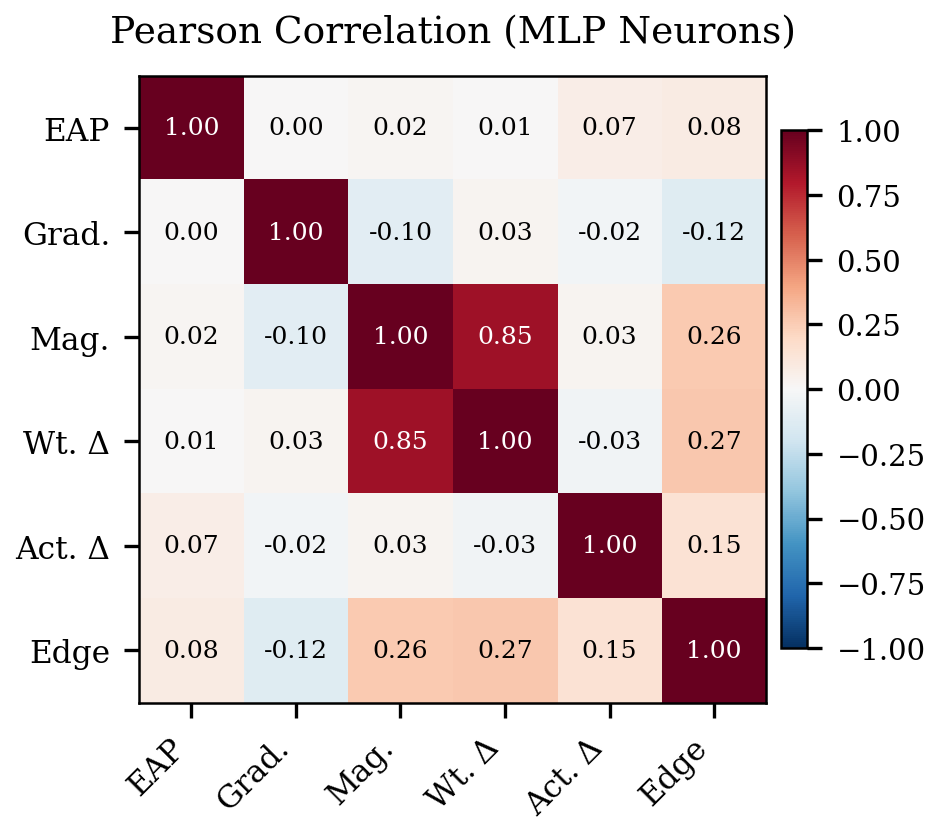
\includegraphics[width=\columnwidth]{figures/figA_correlation.png}
\caption{Pearson correlation across the six signals for all 
239,616 MLP neurons of Gemma-2-2B. Only Magnitude and 
Weight~$\Delta$ are strongly correlated ($r{=}0.85$); all other 
pairs are near-orthogonal ($|r| < 0.27$). Mean off-diagonal 
$|r| = 0.098$.}
\label{fig:corr_heatmap}
\end{figure}

\begin{figure}[t]
\centering
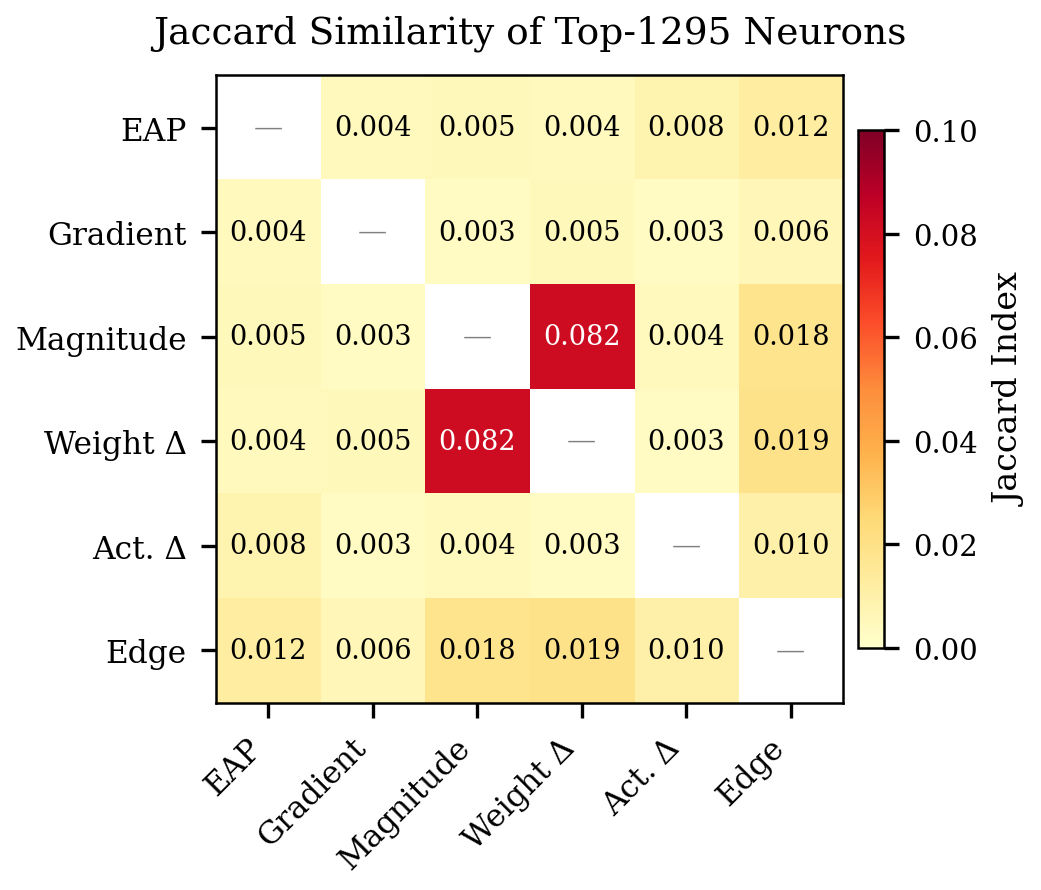
\includegraphics[width=\columnwidth]{figures/figA1_signal_overlap.png}
\caption{Jaccard similarity of the top-1,295 neurons selected 
by each signal. Despite the Pearson correlation between 
Magnitude and Weight~$\Delta$ ($r{=}0.85$), even this pair has 
low top-$k$ overlap (Jaccard $= 0.082$); all other pairs are 
below 0.02. Mean pairwise Jaccard $= 0.012$.}
\label{fig:jaccard}
\end{figure}

\begin{table}[t]
\centering
\small
\resizebox{\columnwidth}{!}{%
\begin{tabular}{lcccccc}
\toprule
 & \textbf{EAP} & \textbf{Grad} & \textbf{Mag} & \textbf{W$\Delta$} & \textbf{Act$\Delta$} & \textbf{Edge} \\
\midrule
EAP &   & .000 & .023 & .007 & .066 & .080 \\
Grad & &   & $-$.104 & .027 & $-$.024 & $-$.125 \\
Mag & & &   & \textbf{.850} & .031 & .260 \\
W$\Delta$ & & & &   & $-$.033 & .269 \\
Act$\Delta$ & & & & &   & .147 \\
Edge & & & & & &   \\
\bottomrule
\end{tabular}}
\caption{Pearson correlation between signals on Gemma-2-2B MLP 
neurons. Mean off-diagonal $|r| = 0.098$.}
\label{tab:corr}
\end{table}

Figures~\ref{fig:corr_heatmap} and~\ref{fig:jaccard} and 
Table~\ref{tab:corr} show why we describe the six signals as 
\emph{complementary} rather than decorrelated. Magnitude and 
Weight~$\Delta$ share 72\% of their variance globally 
($r{=}0.85$), yet their top-$k$ neuron sets overlap by only 
8.2\%; every other pair overlaps by under 2\%. Selection by 
rank therefore draws different neurons from each signal even 
when their raw values are correlated.

The Magnitude and Weight~$\Delta$ correlation is expected: 
neurons with large weights tend to receive large absolute 
updates because optimizer steps scale with gradients, and 
gradients are larger for high-magnitude weights. The rankings 
differ because Magnitude captures importance inherited from 
pretraining while Weight~$\Delta$ captures task-specific 
adaptation: a neuron can have large magnitude and small delta 
(important for general language, untouched by fine-tuning) or 
small magnitude and large delta (recruited by fine-tuning).

\paragraph{Why six signals?}
Low overlap establishes that the signals identify different 
neurons; it does not by itself establish that combining them 
helps compression, and Sections~\ref{sec:selection} 
and~\ref{sec:llama} test that directly. On Gemma-2-2B every 
selection rule, including random, retains 98 to 100\% at the 
main layout, so the question cannot be resolved there. On 
Llama-3-8B three signals (EAP, Gradient, Magnitude) select an 
effective skeleton and three (Weight~$\Delta$, 
Activation~$\Delta$, Edge) do no better than random, while on 
Gemma-2-2B at 4-bit Weight~$\Delta$ was among the best single 
signals and Activation~$\Delta$ the worst 
(Appendix~\ref{app:ablation}). Which signals are effective 
therefore depends on the model, and we have no way to predict 
it in advance. The consensus rule is our answer to that 
uncertainty: it matched the best single signal on both models 
without knowing which one that was. We make no claim that six 
is the right number; each signal we use is cheap relative to 
one forward pass of the base model, and the rule tolerates 
inert signals because a neuron must exceed the threshold on at 
least three.

\paragraph{Why not tier attention heads?}
We quantize all attention heads uniformly rather than tiering 
them like MLP neurons, for two reasons. First, with 208 heads 
against 239,616 neurons, cross-signal consensus has little 
resolution: a threshold applied to 208 components yields very 
coarse tiers. Second, attention precision is not sparse in its 
effect on Gemma-2-2B: with 8-bit attention, every MLP layout 
from 3-bit to 4-bit retains 98 to 100\%, while dropping 
attention to 4-bit with the same skeleton reduces retention to 
77.1\% (Section~\ref{sec:findings}), which indicates that 
attention heads are broadly rather than sparsely important for 
SQL generation. All 8 heads of Layer~0 are classified as 
skeleton by our signals, consistent with the first layer's 
attention handling token routing that the whole task depends on.


\section{Signal Ablation on Gemma-2-2B}
\label{app:ablation}

\begin{figure}[t]
\centering
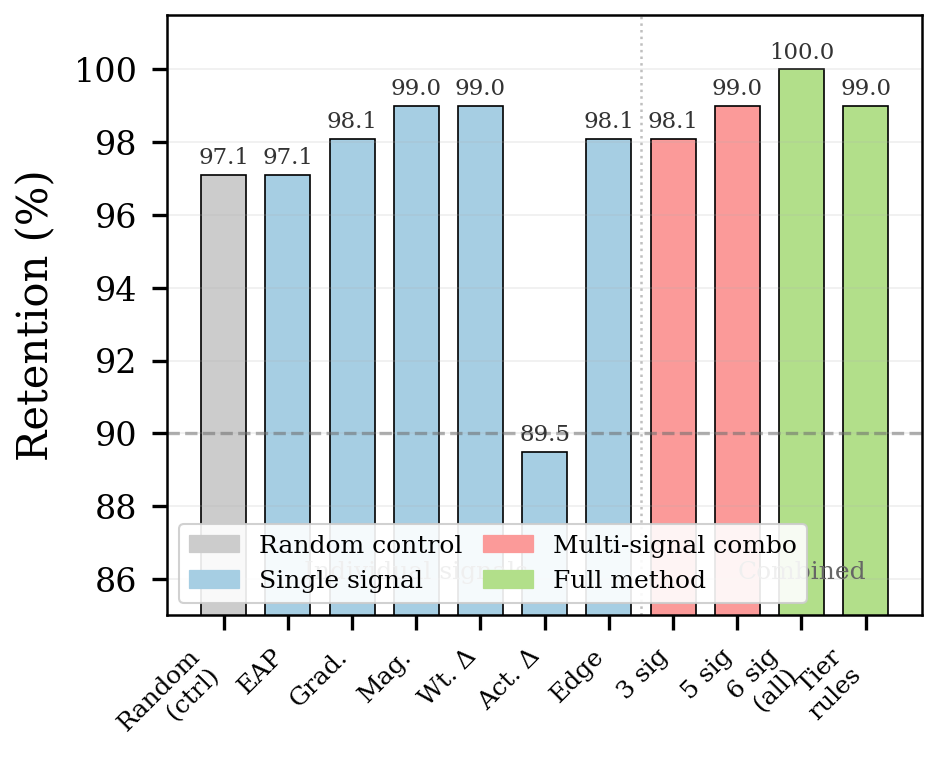
\includegraphics[width=\columnwidth]{figures/figA4_signal_ablation.png}
\caption{Single-signal and combined selection on Gemma-2-2B at 
the c4+a8 layout under the gathered-subset quantizer 
(Table~\ref{tab:full_ablation}). Each bar selects the 
top-1,295 neurons by one signal (blue), by a combination 
(pink), or by the full tier rule (green); gray is one random 
seed. All bars lie between 89.5 and 100\%.}
\label{fig:ablation}
\end{figure}

\begin{table}[t]
\centering
\small
\begin{tabular}{lcc}
\toprule
\textbf{Selection method} & \textbf{Ret.\%} & \textbf{Kept} \\
\midrule
Random (5 seeds) & 98.7$\pm$1.1 & 102 to 105 \\
EAP & 97.1 & 102/105 \\
Gradient & 98.1 & 103/105 \\
Magnitude & 99.0 & 104/105 \\
Weight $\Delta$ & 99.0 & 104/105 \\
Activation $\Delta$ & 89.5 & 94/105 \\
Edge importance & 98.1 & 103/105 \\
\midrule
EAP + Gradient & 98.1 & 103/105 \\
EAP + Weight $\Delta$ & 96.2 & 101/105 \\
EAP + Activation $\Delta$ & 93.3 & 98/105 \\
Gradient + Magnitude & 97.1 & 102/105 \\
Magnitude + Weight $\Delta$ & 98.1 & 103/105 \\
EAP + Gradient + Magnitude & 98.1 & 103/105 \\
Four signals (+ Weight $\Delta$) & 95.2 & 100/105 \\
Five signals (+ Activation $\Delta$) & 99.0 & 104/105 \\
Six-signal top-$k$ union & 100.0 & 105/105 \\
Full tier rule & 99.0 & 104/105 \\
\bottomrule
\end{tabular}
\caption{Signal ablation on Gemma-2-2B. Every row protects 
exactly 1,295 neurons at 16-bit with all other MLP weights at 
4-bit and attention at 8-bit, using the gathered-subset 
quantizer of the original submission 
(Appendix~\ref{app:reliability}). Combinations select the 
top-1,295 by summed normalized score.}
\label{tab:full_ablation}
\end{table}

Figure~\ref{fig:ablation} and Table~\ref{tab:full_ablation} 
give the per-signal picture on Gemma-2-2B. Each row selects 
the top-1,295 neurons (the size of the tier-rule skeleton) by 
the stated signal or combination and protects them at 16-bit 
with every other MLP neuron at 4-bit and attention at 8-bit. 
These runs use the gathered-subset quantizer of the original 
submission, which adds grouping variance in the down 
projection (Appendix~\ref{app:reliability}); we retain them 
because they are the only per-signal measurements on this 
model, and the pattern they show is corroborated on Llama-3-8B 
under the corrected quantizer (Section~\ref{sec:llama}).

Three observations survive the noise. First, at this layout 
selection barely matters: random protection over five seeds 
averages 98.7\%, and twelve of the sixteen rows are within two 
samples of it. Second, the one clear outlier is 
Activation~$\Delta$ alone at 89.5\%, eight to ten points below 
the other single signals; activation deltas are noisy because upstream weight changes propagate to downstream neurons that are not themselves 
task-critical. Third, Weight~$\Delta$ alone is among the best 
signals here (99.0\%), whereas on Llama-3-8B it is 
indistinguishable from random (Table~\ref{tab:llama}). The 
effective single signal is therefore model-dependent, which is 
the empirical basis for using a consensus rule rather than any 
one signal. The combinations do not improve monotonically with 
the number of signals (four signals score below three), and the 
six-signal union at 100.0\% is one sample above the tier rule 
at 99.0\%; neither difference is interpretable at $n{=}105$.

Under the corrected quantizer at the main c3+a8 layout, 
Table~\ref{tab:main}(b) repeats the comparison for none, 
random, a TaCQ-style vulnerability selection, the percentile 
rule, and the tier rule; all lie between 98.1 and 100.0\%.


\section{Quantizer Sensitivity and Confidence Intervals}
\label{app:reliability}

\paragraph{The gathered-subset artifact.}
The original submission quantized protected and unprotected 
neurons by gathering the corresponding rows of the gate and up 
projections and columns of the down projection into a 
sub-matrix and quantizing that sub-matrix per-group. For the 
down projection the number of unprotected columns is not a 
multiple of the group size, so the group boundaries shift with 
every different protection set. At 3-bit this shifts the 
min-max grid of most groups and produces retention differences 
that depend on which neurons were selected but not on their 
importance. Table~\ref{tab:artifact} shows the effect: under 
the gathered quantizer, five random skeletons at c3+a8 span 
69.5 to 99.0\%, and one seed at c3+a4 falls to 60.0\%. Under 
the corrected quantizer of Section~\ref{sec:quant}, which 
quantizes the full matrix once and restores protected neurons 
afterwards, the same five seeds span 98.1 to 99.0\% and are 
indistinguishable from protecting nothing. The reliability 
advantage reported in the original submission was this 
artifact, and all results in the present version use the 
corrected quantizer.

\begin{table}[t]
\centering
\small
\resizebox{\columnwidth}{!}{%
\begin{tabular}{llcc}
\toprule
\textbf{Layout} & \textbf{Selection} & \textbf{Gathered} & \textbf{Aligned} \\
\midrule
c3+a8 & None & \multicolumn{1}{c}{n/a} & 98.1 \\
c3+a8 & Random (5 seeds) & 91.6$\pm$12.4 & 98.7$\pm$0.5 \\
c3+a8 & Tier-rule skeleton & 97.1 & 100.0 \\
\midrule
c3+a4 & None & \multicolumn{1}{c}{n/a} & 95.2 \\
c3+a4 & Random (5 / 3 seeds) & 84.4$\pm$14.3 & 94.9$\pm$0.5 \\
c3+a4 & Tier-rule skeleton & 94.3 & 95.2 \\
\bottomrule
\end{tabular}}
\caption{Retention on Gemma-2-2B ($n{=}105$) under the 
gathered-subset quantizer of the original submission and the 
aligned protect-by-restore quantizer used throughout this 
version. Random rows report mean and standard deviation over 
seeds (five gathered; five and three aligned for c3+a8 and 
c3+a4). Selection-dependent variance disappears once the 
grouping is held fixed.}
\label{tab:artifact}
\end{table}

\paragraph{Determinism.}
Given the same checkpoints, analysis samples, and hardware, 
signal values, tier assignments, quantized weights, and greedy 
decoding are deterministic: re-running the c4+a8 configuration 
and the GPTQ uniform 4-bit configuration on the same machine 
reproduced 101 of 105 in both cases. Determinism does not 
extend across platforms for GPTQ, whose Hessian inverse is 
numerically fragile (Appendix~\ref{app:gptq}); round-to-nearest 
results reproduced exactly between the February and September 
runs on different GPUs.

\paragraph{Confidence intervals.}
\label{app:ci}
Table~\ref{tab:ci} reports 95\% Wilson score intervals for the 
configurations in Tables~\ref{tab:main} and~\ref{tab:llama}. On 
Gemma-2-2B, the c3+a8 layout is separated from uniform 4-bit 
and from every GPTQ 3-bit configuration at the interval level, 
but its interval overlaps that of the same layout with no 
skeleton, which is why Section~\ref{sec:selection} makes no 
selection claim on this model. On Llama-3-8B, the skeleton and 
no-skeleton intervals do not overlap.

\begin{table}[t]
\centering
\small
\begin{tabular}{lcc}
\toprule
\textbf{Configuration} & \textbf{Ret.\%} & \textbf{95\% CI} \\
\midrule
\multicolumn{3}{l}{\textit{Gemma-2-2B ($n{=}105$)}} \\
Uniform 4-bit & 75.2 & 66.2 to 82.5 \\
Uniform 3-bit & 87.6 & 80.0 to 92.6 \\
GPTQ uniform 4-bit & 96.2 & 90.6 to 98.5 \\
GPTQ uniform 3-bit & 77.1 & 68.2 to 84.1 \\
MLP@4 + attn@8, no skeleton & 100.0 & 96.5 to 100.0 \\
CircuitTier c4+a8 & 99.0 & 94.8 to 99.8 \\
MLP@3 + attn@8, no skeleton & 98.1 & 93.3 to 99.5 \\
CircuitTier c3+a8 & 100.0 & 96.5 to 100.0 \\
GPTQ MLP@3 + attn@8 & 81.9 & 73.5 to 88.1 \\
Four-tier c4+a8 (with pruning) & 91.4 & 84.5 to 95.4 \\
\midrule
\multicolumn{3}{l}{\textit{Llama-3-8B ($n{=}894$)}} \\
Uniform 4-bit & 77.1 & 74.2 to 79.7 \\
Gradient skeleton & 91.9 & 89.9 to 93.5 \\
Six-signal skeleton & 91.5 & 89.5 to 93.2 \\
\bottomrule
\end{tabular}
\caption{95\% Wilson score intervals for retention.}
\label{tab:ci}
\end{table}


\section{GPTQ Analysis}
\label{app:gptq}

\begin{figure}[t]
\centering
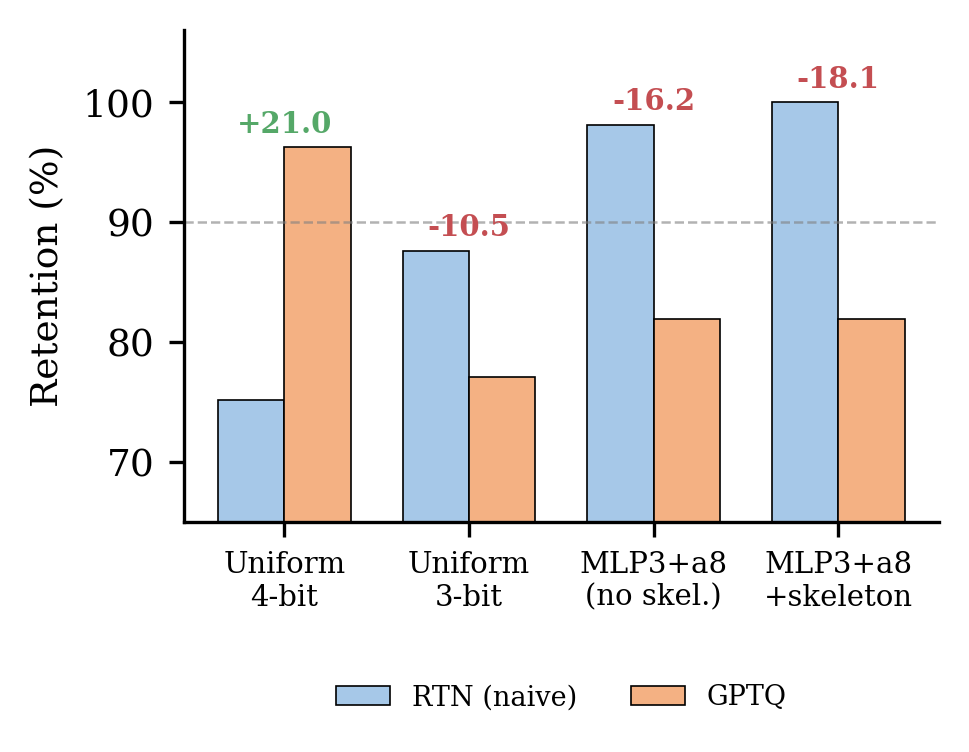
\includegraphics[width=\columnwidth]{figures/fig7_gptq_vs_rtn.png}
\caption{Round-to-nearest versus GPTQ on Gemma-2-2B ($n{=}105$), 
same per-group grid in both. GPTQ helps uniform 4-bit by 21 
points and hurts every 3-bit layout by 10 to 18 points, with 
and without the skeleton.}
\label{fig:gptq}
\end{figure}

\paragraph{Implementation.}
We use the standard GPTQ procedure 
\cite{frantar2023gptqaccurateposttrainingquantization}: 
Hessians $H = X^\top X$ are accumulated over 128 analysis 
samples for every linear projection, damped by 0.01 times the 
mean diagonal, and inverted by Cholesky decomposition; columns 
are quantized sequentially in blocks of 128 with error 
propagated to later columns through the inverse Hessian. Each 
column is quantized with the same asymmetric min-max grid over 
groups of 128 weights as our RTN baseline, so the two methods 
differ only in error compensation. For protected neurons we 
quantize the full matrix and restore their weights afterwards, 
exactly as for RTN.

\paragraph{Results.}
Figure~\ref{fig:gptq} shows that GPTQ raises uniform 4-bit 
retention from 75.2\% to 96.2\% but lowers uniform 3-bit from 
87.6\% to 77.1\%, MLP@3 with 8-bit attention from 98.1\% to 
81.9\%, and the same layout with the skeleton restored from 
100\% to 81.9\%. The last two are identical to the sample, so 
at 3-bit the degradation is independent of neuron protection.

\paragraph{Contamination is not the mechanism.}
The original submission attributed GPTQ's degradation of 
protected layouts to error being redistributed into the 16-bit 
skeleton columns of the down projection. We measured this 
directly (Table~\ref{tab:gptq_dw}) under the submission's 
sub-matrix implementation, in which skeleton columns are 
excluded from quantization but do receive redistributed error. 
Skeleton columns of the down projection are perturbed by a 
mean $|\Delta w|$ of 0.00029, against 0.00074 for quantized 
columns; skeleton rows of the gate and up projections are 
untouched. Redistribution into protected weights is real but 
less than half the size of ordinary quantization error, and the 
degradation persists when protected weights are fully restored, 
so contamination cannot explain it.

\begin{table}[t]
\centering
\small
\begin{tabular}{lcc}
\toprule
\textbf{Neuron group} & \textbf{All projections} & \textbf{Down only} \\
\midrule
Skeleton (1,295) & 0.00010 & 0.00029 \\
Non-skeleton (238,321) & 0.00078 & 0.00074 \\
\bottomrule
\end{tabular}
\caption{Mean $|\Delta w|$ per weight after GPTQ at the c4+a8 
layout under the sub-matrix implementation, by neuron group. 
Skeleton gate and up rows are not quantized, which lowers the 
all-projection mean; the down-only column is the relevant 
comparison.}
\label{tab:gptq_dw}
\end{table}

\paragraph{Sensitivity.}
GPTQ's inverse-Hessian step is numerically fragile in this 
setting: Hessian condition numbers reach $10^{5}$ for MLP 
projections and $10^{13}$ for attention projections. 
Table~\ref{tab:gptq_sens} shows the consequences. Uniform 4-bit 
gives 96.2\% at damping 0.01 and 88.6\% at damping 0.1 on the 
same machine, and 79.0\% with identical code, calibration set, 
and damping on a different GPU and framework build in our 
original submission; the sub-matrix c4+a8 layout moved from 
89.5\% to 98.1\% across the same change. Round-to-nearest 
results reproduced exactly across both machines. We therefore 
treat the sign of GPTQ's effect at 3-bit as robust (it 
degraded 3-bit layouts in every run on both machines) and its 
4-bit magnitude as indicative.

\begin{table}[t]
\centering
\small
\begin{tabular}{lcc}
\toprule
\textbf{GPTQ configuration} & \textbf{Feb.} & \textbf{Sept.} \\
\midrule
Uniform 4-bit, damp 0.01 & 79.0 & 96.2 \\
Uniform 4-bit, damp 0.1 & n/a & 88.6 \\
Uniform 3-bit, damp 0.01 & 81.9 & 77.1 \\
Sub-matrix c4+a8, damp 0.01 & 89.5 & 98.1 \\
\midrule
RTN uniform 4-bit & 75.2 & 75.2 \\
RTN c4+a8 (sub-matrix) & 96.2 & 96.2 \\
\bottomrule
\end{tabular}
\caption{GPTQ retention on Gemma-2-2B ($n{=}105$) across 
damping and hardware, with the same code and calibration set. 
Feb.\ runs used an A40, Sept.\ runs an RTX PRO 4500. RTN rows 
show the reproducibility of the non-GPTQ pipeline. Repeated 
runs on one machine are identical.}
\label{tab:gptq_sens}
\end{table}

\paragraph{Interpretation.}
We do not have a verified mechanism for the 3-bit degradation. 
One hypothesis consistent with the data is that at 3-bit the 
per-column residual is large relative to the group's min-max 
range, so the sequential corrections pushed into later columns 
frequently move them across grid boundaries, compounding rather 
than cancelling error, whereas at 4-bit the corrections are 
small enough to act as intended. Testing this requires 
per-column error traces and is left to future work. The 
practical conclusion is narrower than the original submission's: 
in our setting, GPTQ should not be combined with 3-bit min-max 
grouping, where plain round-to-nearest is 16 to 18 points 
better, and GPTQ's benefit at 4-bit should be verified on the 
deployment hardware.

\section{Threshold Sensitivity}
\label{app:threshold}

\begin{table}[t]
\centering
\small
\begin{tabular}{lccc}
\toprule
\textbf{Rule} & \textbf{Skeleton} & \textbf{\%} & \textbf{Ret.\%} \\
\midrule
\multicolumn{4}{l}{\textit{Absolute $\tau$, four-tier c4+a8, gathered quantizer}} \\
$\tau{=}0.25$ & 4,074 & 1.70 & 95.2 \\
$\tau{=}0.30$ & 1,295 & 0.54 & 96.2 \\
$\tau{=}0.35$ & 339 & 0.14 & 96.2 \\
\midrule
\multicolumn{4}{l}{\textit{Percentile $P$, c3+a8, aligned quantizer}} \\
$P{=}99$ & 137 & 0.06 & 99.0 \\
$P{=}99.5$ & 51 & 0.02 & 99.0 \\
$\tau{=}0.30$ (reference) & 1,295 & 0.54 & 100.0 \\
None (reference) & 0 & 0.00 & 98.1 \\
\bottomrule
\end{tabular}
\caption{Threshold sensitivity on Gemma-2-2B ($n{=}105$). The 
absolute sweep uses the four-tier layout and quantizer of the 
original submission; the percentile rows use the main layout 
of this version.}
\label{tab:threshold}
\end{table}

Table~\ref{tab:threshold} varies the skeleton threshold over 
a twelvefold range of skeleton size, from 339 to 4,074 
neurons, and retention moves by one sample. Under the 
percentile rule at the main layout, skeletons of 51 and 137 
neurons retain 99.0\%, one sample below the 1,295-neuron 
skeleton and one above no skeleton. On this model the threshold 
is not a sensitive parameter because, as 
Section~\ref{sec:selection} shows, selection itself is not: 
there is nothing in the interval for the threshold to get 
wrong. The prunable threshold $\tau'{=}0.1$ identifies 48 
neurons on which all six signals are low; zeroing them costs 
eight samples at c4+a8 (Appendix~\ref{app:tiers}), so we do not 
use it.

\section{Tier Ablation}
\label{app:tiers}

\begin{table}[t]
\centering
\small
\begin{tabular}{lcc}
\toprule
\textbf{Layout} & \textbf{c4+a8} & \textbf{c3+a8} \\
\midrule
No skeleton & 100.0 & 98.1 \\
Two-tier (skeleton@16) & 99.0 & 100.0 \\
+ supporting@8 & 99.0 & n/a \\
+ prunable@0 (four-tier) & 91.4 & 99.0 \\
\bottomrule
\end{tabular}
\caption{Tier ablation on Gemma-2-2B ($n{=}105$), aligned 
quantizer. Rows add tiers cumulatively: the two-tier layout 
restores the 1,295 skeleton neurons; the third row additionally 
holds the 23 supporting neurons at 8-bit; the fourth 
additionally zeroes the 48 prunable neurons.}
\label{tab:tier_ablation}
\end{table}

Table~\ref{tab:tier_ablation} adds the tiers of 
Section~\ref{sec:tiers} one at a time. The supporting tier 
changes nothing: with and without it the c4+a8 layout retains 
99.0\%, and merging supporting neurons into the compressible 
tier under the gathered quantizer gave 97.1\% against 96.2\% 
for the full four-tier layout. The prunable tier is harmful: 
zeroing 48 neurons drops c4+a8 from 99.0\% to 91.4\%, with six 
of the nine lost samples in CS1, while at c3+a8 the same 
zeroing costs one sample. The recommended layout is therefore 
two tiers, skeleton and everything else.

\paragraph{VulnSplit.}
The original submission subdivided the compressible tier by a 
TaCQ-style per-neuron vulnerability score, assigning the least 
vulnerable 50\% or 75\% of compressible neurons to 3-bit and 
the rest to 4-bit. Under the aligned quantizer both splits 
retain 95.2\% (at 4.37 and 4.17 bits), below the plain c3+a8 
layout at 3.97 bits (100\%) and below MLP@4 with attention at 
8-bit (100\% at 4.73 bits). The subdivision is dominated on 
both axes and is not part of the method.

\section{Layer Distribution}
\label{app:layers}

\begin{figure}[t]
\centering
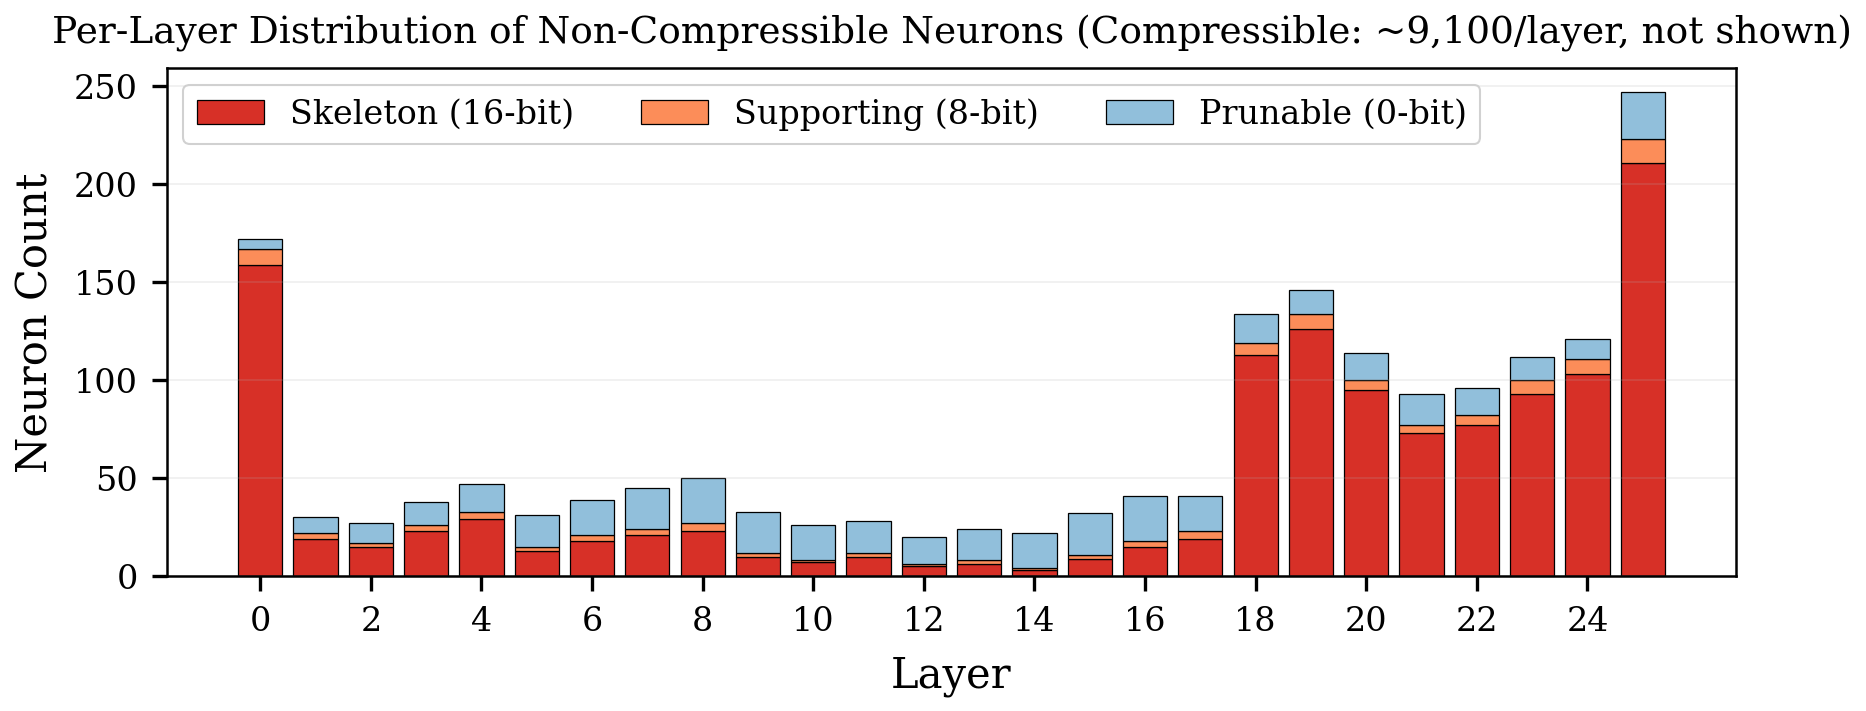
\includegraphics[width=\columnwidth]{figures/figA3_layer_distribution.png}
\caption{Per-layer distribution of skeleton, supporting, and 
prunable neurons on Gemma-2-2B. Skeleton neurons (red) 
concentrate in Layer~0 and Layers 18 to 25. The compressible 
majority (about 9,100 per layer) is omitted.}
\label{fig:layer_dist}
\end{figure}

Skeleton neurons are distributed bimodally across layers 
(Figure~\ref{fig:layer_dist}): Layer~0 holds about 160 and 
Layers 18 to 25 between roughly 90 and 245 each, while the 
middle layers (10 to 16) hold few. All 8 attention heads of 
Layer~0 are classified as skeleton.

This pattern is interpretable for SQL generation. The early 
layers, especially Layer~0, perform token processing and 
schema recognition, identifying table names, column names, 
and SQL keywords in the prompt; the model must parse the input 
before it can generate. The final layers convert the internal 
representation into syntactically correct SQL tokens. The 
middle layers, which handle general language processing, were 
largely unchanged by fine-tuning. On Llama-3-8B the skeleton 
concentrates in the last five layers (27 to 31); the late-layer 
component replicates, the Layer~0 component does not.

\section{Per-Complexity Results}
\label{app:percs}

\begin{table}[t]
\centering
\small
\setlength{\tabcolsep}{3pt}
\resizebox{\columnwidth}{!}{%
\begin{tabular}{lccccc|c}
\toprule
\textbf{Configuration} & \textbf{CS1} & \textbf{CS2} & \textbf{CS3} & \textbf{CS4} & \textbf{CS5} & \textbf{All} \\
\midrule
Baseline & 100 & 100 & 100 & 100 & 100 & 100.0 \\
Uniform 4-bit & 57 & 84 & 87 & 67 & 86 & 75.2 \\
Uniform 3-bit & 100 & 84 & 83 & 87 & 79 & 87.6 \\
GPTQ uniform 3-bit & 100 & 64 & 74 & 73 & 64 & 77.1 \\
MLP@3 + attn@8, no skeleton & 100 & 92 & 100 & 100 & 100 & 98.1 \\
CircuitTier c3+a8 & 100 & 100 & 100 & 100 & 100 & 100.0 \\
GPTQ MLP@3 + attn@8 & 100 & 80 & 83 & 67 & 64 & 81.9 \\
Four-tier c4+a8 (with pruning) & 79 & 100 & 96 & 93 & 93 & 91.4 \\
\bottomrule
\end{tabular}}
\caption{Retention (\%) by SQL complexity level on Gemma-2-2B 
(CS1 simplest, CS5 most complex). Baseline-correct samples: 
CS1 = 28, CS2 = 25, CS3 = 23, CS4 = 15, CS5 = 14; CS4 and CS5 
are small and per-level numbers should be read with caution.}
\label{tab:per_cs}
\end{table}

Two patterns stand out in Table~\ref{tab:per_cs}. Uniform 
4-bit degrades CS1, the simplest queries, most (57\%), and 
zeroing the prunable tier at c4+a8 also loses its samples 
mainly in CS1 (79\%): the simplest queries appear to depend on 
a small, precise set of weights whose disruption is not 
compensated elsewhere. GPTQ at 3-bit, by contrast, keeps CS1 
intact and loses samples across CS2 to CS5. The c3+a8 layout 
retains every sample at every level.

\section{General Capability}
\label{app:ppl}

\begin{table}[t]
\centering
\small
\begin{tabular}{lcc}
\toprule
\textbf{Configuration} & \textbf{PPL} & \textbf{Ratio} \\
\midrule
Fine-tuned 16-bit & 32.3 & 1.00$\times$ \\
Uniform 4-bit & 36.5 & 1.13$\times$ \\
MLP@4 + attn@8, no skeleton & 33.8 & 1.05$\times$ \\
CircuitTier c4+a8 & 33.8 & 1.05$\times$ \\
MLP@3 + attn@8, no skeleton & 47.4 & 1.47$\times$ \\
CircuitTier c3+a8 & 47.6 & 1.47$\times$ \\
\bottomrule
\end{tabular}
\caption{WikiText-2 test perplexity of the fine-tuned 
Gemma-2-2B under each layout, computed over 2,048-token windows 
with a BOS token prepended to each window.}
\label{tab:ppl}
\end{table}

Table~\ref{tab:ppl} reports general-domain perplexity on 
WikiText-2 \cite{merity2016pointersentinelmixturemodels}. The 
fine-tuned model starts at 32.3, well above the base model, 
because SQL fine-tuning has already traded general capability 
for the task. The 4-bit layouts with 8-bit attention degrade 
perplexity less than uniform 4-bit (1.05$\times$ against 
1.13$\times$), so at 4-bit the layout costs nothing in general 
capability. The 3-bit MLP layouts degrade it by 1.47$\times$; 
this is the price of the 4.03$\times$ headline configuration, 
and it is the same with or without the skeleton. For 
multi-purpose deployment, MLP@4 with 8-bit attention at 
3.38$\times$ is the better operating point.

\section{Compression Wall on Llama-3-8B}
\label{app:wall}

\begin{table}[t]
\centering
\small
\setlength{\tabcolsep}{4pt}
\begin{tabular}{lcc}
\toprule
\textbf{skel / supp / MLP / attn, $g$} & \textbf{Ratio} & \textbf{Ret.\%} \\
\midrule
16 / 8 / 4 / 4, 128 & 3.84$\times$ & 98 \\
16 / 4 / 3 / 3, 128 & 5.20$\times$ & 59 \\
16 / 4 / 3 / 3, 64 & 5.20$\times$ & 68 \\
8 / 4 / 3 / 3, 64 & 5.25$\times$ & 73 \\
16 / 8 / 2 / 4, 32 & 6.13$\times$ & 27 \\
16 / 4 / 2 / 3, 64 & 6.95$\times$ & 10 \\
16 / 8 / 1 / 4, 32 & 8.71$\times$ & 0 \\
\bottomrule
\end{tabular}
\caption{Representative rows of a 22-configuration sweep on 
Llama-3-8B ($n{=}100$, earlier protocol, retention relative to 
the 16-bit model). Columns give the bit-widths of skeleton, 
supporting, and compressible MLP neurons and of attention, and 
the quantization group size. No configuration above 4.6$\times$ 
retains more than 73\%.}
\label{tab:wall}
\end{table}

An earlier sweep of 22 layouts between 4.6$\times$ and 
9.3$\times$ on Llama-3-8B ($n{=}100$, under the original 
quantizer and evaluation) found a hard wall near 5$\times$: 
every layout with 2-bit MLPs collapses regardless of skeleton 
size, supporting precision, or group size, and the best 
3-bit-MLP layout retains 73\% at 5.25$\times$ 
(Table~\ref{tab:wall}). Smaller quantization groups help at the 
margin (59\% to 68\% from $g{=}128$ to $g{=}64$) but do not 
move the wall. Quantization-aware fine-tuning for 100 steps did not help even at 4-bit (uniform 56\% to 54\%, skeleton layout 96\% to 93\%, 
$n{=}100$).


\section{Future Directions}
\label{app:future}

\paragraph{Scale and generalization.}
Validating the headroom hypothesis on a third model family and 
across a 7B to 70B range on one task is the most important next 
step: measure uniform 4-bit headroom first, then skeleton 
recovery. Diverse tasks (summarization, code generation, 
mathematical reasoning) would test whether the effective 
signals are a property of the task, the model, or the 
fine-tune. We no longer expect larger models to have sparser 
skeletons as a rule; Llama-3-8B's skeleton (0.46\%) is close to 
Gemma-2-2B's (0.54\%) under different rules, and skeleton size 
did not predict retention on either.

\paragraph{Why the effective signals differ.}
Weight delta selects an effective skeleton on Gemma-2-2B and 
not on Llama-3-8B, while EAP, gradient, and magnitude work on 
both. Understanding what makes a signal informative for a given 
fine-tune would let the consensus rule be replaced by a 
principled choice, or confirm that consensus is the right 
default.

\paragraph{Multi-task circuits.}
When a model is fine-tuned on multiple tasks, whether task 
skeletons overlap or are disjoint decides whether one protected 
set can serve several capabilities at once or whether each 
costs its own share of the precision budget. Mapping these 
interactions is both a compression and an interpretability 
question.

\paragraph{Continual fine-tuning.}
If a model is fine-tuned first on SQL and then on another 
task, does the second fine-tune overwrite the first skeleton? 
Re-extracting signals after each stage would track how the 
skeleton moves and whether earlier capabilities can be 
protected during later training.

\paragraph{Learned thresholds.}
On Gemma-2-2B the threshold was insensitive because selection 
was; on a model with headroom a validation-set search for the 
smallest skeleton that reaches a target retention would be 
informative, and the percentile formulation gives it a single 
scalar to search over.

\paragraph{GPTQ at low precision.}
The 3-bit degradation is robust across platforms and 
unexplained. Per-column error traces would test the 
grid-crossing hypothesis of Appendix~\ref{app:gptq}, and the 
result would say whether error compensation can be made to 
work below 4-bit with min-max grouping or should be avoided 
there.

\paragraph{Inference integration.}
Realizing the bit savings as latency requires mixed-precision 
kernels. The two-tier layout maps directly to existing 4-bit 
engines with the skeleton stored separately, which is the 
natural first deployment; 3-bit MLPs need kernel support that 
current engines lack.

\end{document}